\documentclass[11pt,a4paper]{article}
\author{TalentSprint}
\date{}
\usepackage{graphicx}
\usepackage{verbatim}
\usepackage{array}
\usepackage{caption}
\usepackage{enumitem}
\usepackage{xcolor}
\usepackage[tikz]{bclogo}
\usepackage{textcomp}
\usepackage{listings}
\usepackage{multicol}
\usepackage{float}
\usepackage{seqsplit} 
\usepackage{setspace}
\usepackage{soul}
\usepackage{latexsym}
\lstset{language=Java,numbers=left, numberstyle=\tiny, numbersep=10pt, showstringspaces=false, breaklines=true,keepspaces=true, columns=flexible}
\usepackage{fancyhdr}
\headheight=14pt
\lhead{\nouppercase{}}
\rhead{\nouppercase{\leftmark}}

\graphicspath{{../Images/}}


\begin{comment}
\setcounter{tocdepth}{1}
\setlength\parindent{0pt}
\parskip=4pt
\def\AnswerBox{\fbox{\begin{minipage}{4in}\hfill\vspace{0.5in}\end {minipage}}}

\thispagestyle{empty}
\vspace{1.5pc}
\topskip0pt
\vspace*{\fill}
\centerline{\sc \Huge Version Control System}
\vspace{2pc}
\vspace*{\fill}
\centerline{Prepared by TalentSprint WISE Team} 
\setcounter{page}{1}
\pagestyle{fancy}
\end{comment}


%========================================================================

% Lengths and widths
\addtolength{\textwidth}{2.5cm}
\addtolength{\hoffset}{0cm}
\setlength{\headsep}{-12pt} % Reduce space between header and content
\setlength{\headheight}{85pt} % If less, LaTeX automatically increases it
\renewcommand{\footrulewidth}{2pt} % Remove footer line
\renewcommand{\headrulewidth}{1pt} % Remove header line
\renewcommand{\seqinsert}{\ifmmode\allowbreak\else\-\fi} % Hyphens in seqsplit
% This two commands together give roughly
% the right line height in the tables
\renewcommand{\arraystretch}{1.3}
\onehalfspacing



% Commands
\newcommand{\SetRowColor}[1]{\noalign{\gdef\RowColorName{#1}}\rowcolor{\RowColorName}} % Shortcut for row colour
\newcommand{\mymulticolumn}[3]{\multicolumn{#1}{>{\columncolor{white}}#2}{#3}} % For coloured multi-cols
\newcolumntype{x}[1]{>{\raggedright}p{#1}} % New column types for ragged-right paragraph columns
\newcommand{\tn}{\tabularnewline} % Required as custom column type in use

% Font and Colours
\definecolor{HeadBackground}{HTML}{333333}
\definecolor{FootBackground}{HTML}{666666}
\definecolor{TextColor}{HTML}{333333}
\definecolor{DarkBackground}{HTML}{6B8E23} %{FD1AA8}
\definecolor{LightBackground}{HTML}{E8FED8} %D3FDC8
\definecolor{tit}{HTML}{FF6600}
\renewcommand{\familydefault}{\sfdefault}
\color{TextColor}
 \headsep = 25pt
% Header and Footer
\pagestyle{fancy}
\usepackage[headheight=110pt]{geometry}
\fancyhf{}% Clear header/footer

\fancyhead[r]{
\includegraphics[width = 4cm, height = 2cm]{TS-Logo.png}\hspace{0cm}}

%=================================TITLE=====================================
\fancyhead[l]{{\bf{\textcolor{tit}{\textrm{\large{Exceptions \& IO}}}}}}
%===========================================================================

\renewcommand{\headrulewidth}{0.4pt}% Default \headrulewidth is 0.4pt
\renewcommand{\footrulewidth}{0.4pt}% Default \footrulewidth is 0pt

\rfoot{Page \thepage}
\lfoot{COPYRIGHT \textcopyright TALENTSPRINT, 2015. ALL RIGHTS RESERVED.}



\begin{document}



As human beings , we commit many errors. A software engineer may also commit several errors while designing the project or developing the code. These errors are also called `bugs' and the process of removing them is called `debugging'. Let us take a look at different types of errors that are possible in a program.

\subsection*{Errors in a Java program}
There are basically three types of errors in the java program
\begin{description}
\item[Compile-time errors] are syntactical errors found in the code, due to which a program fails to compile. For example, forgetting a semicolon at the end of a Java statement, or writing a statement without proper syntax will result in compile-time error.
\item[Run-time errors] represent inefficiency of the computer system to execute a particular statement. For example, insufficient memory to store something or inability of the microprocessor to execute some statement come under run-time errors.
\item[Logical errors] depict flaws in the logic of the program. The programmer might be using wrong formula or the design of the program itself is wrong. Logical errors are not detected either by Java compiler or JVM. The programmer is soley responsible for them.
\end{description}
\vfill{\ }
\begin{figure}[H]
 \begin{center}
   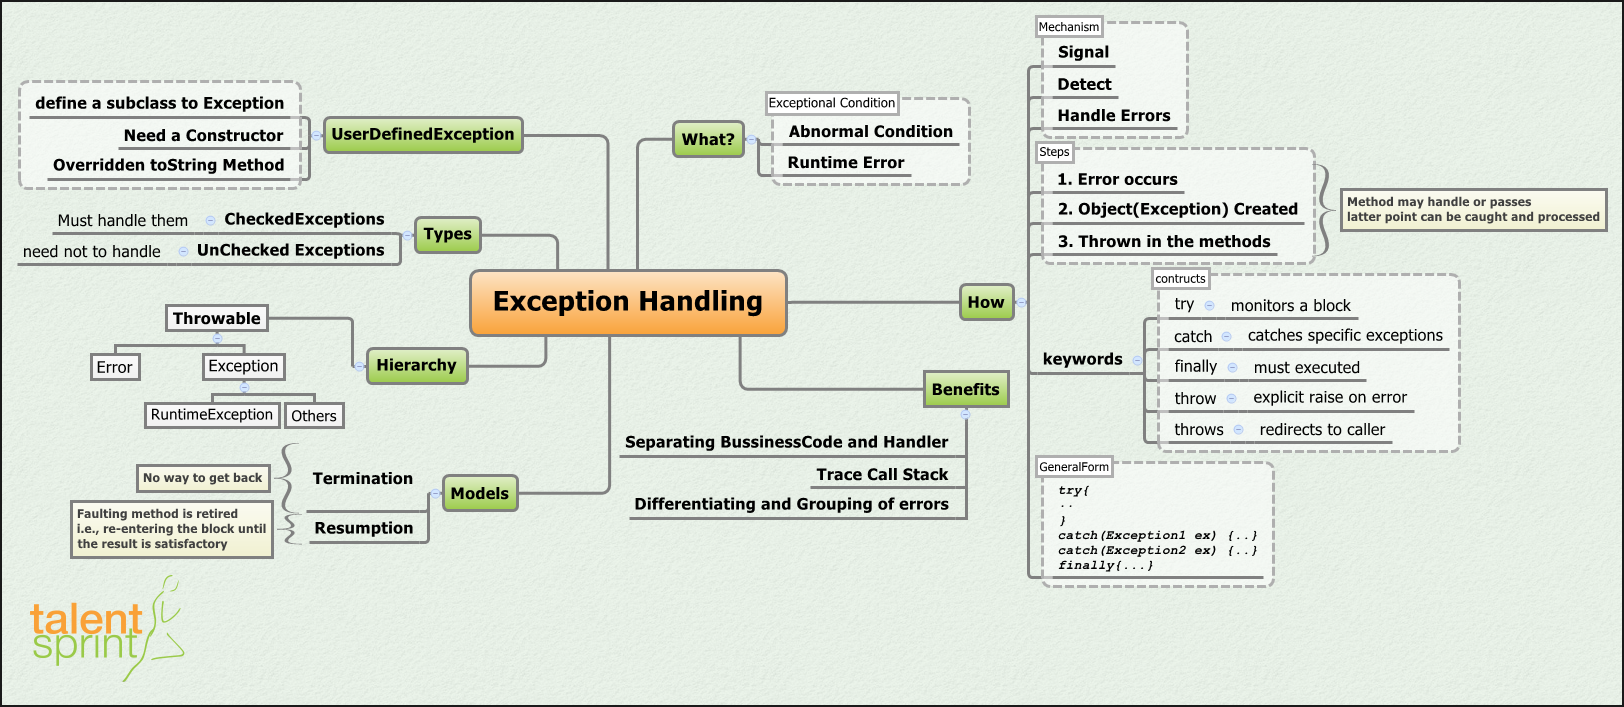
\includegraphics[angle=90,height=19cm, width=13cm]{ExceptionHandling.png}
 \end{center}
 \end{figure}
\section*{Exceptions}
An \texttt{Exception} is a runtime error. Then there raises a doubt, can't I call a compile time error an Exception? The answer is , ``No you cannot call a compile-time errors as exceptions''. They come under errors. All exceptions occur only at runtime but some exceptions are detected at compile time and some others at runtime. The exceptions that are checked at compilation time by the Java compiler are called `checked exceptions' while the exceptions that are checked by the JVM are called `unchecked exceptions'.

Unchecked exceptions and errors are considered as unrecoverable and the programmer cannot do any thing when they occur. The programmer can write a Java program with unchecked exceptions and errors and can compile the program. He can see their effect only when he runs the program. So, Java compiler allows him to write a Java program without handling the unchecked exceptions and errors. In case of checked exceptions, the programmer should either handle them or throw them without handling them. He cannot simply ignore them, as Java compiler will remind him of them. Let us now consider a statement

All exceptions are declared as classes in Java. Of course, everything is a class in Java. Even the errors are also represented by classes. 
All these classes are descended from a super class called \textbf{Throwable}, as shown below.
\begin{figure}[H]
 \begin{center}
   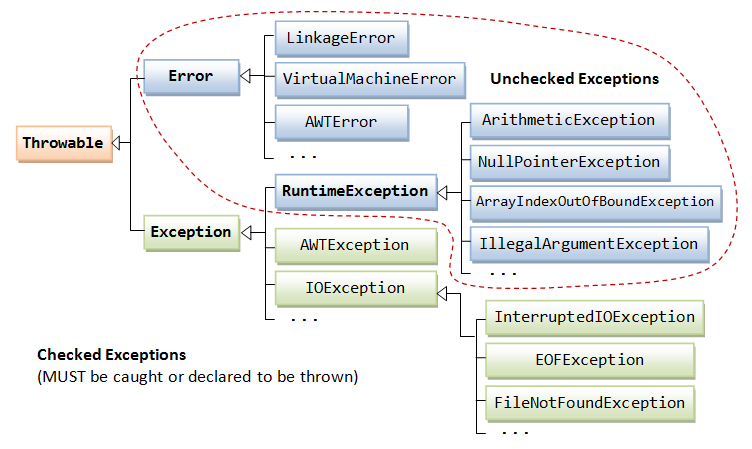
\includegraphics[height=09cm, width=12cm]{ExceptionClasses.png}
 \end{center}
 \end{figure}
 
\begin{lstlisting}[numbers=none]
public static void main(String args[]) throws IOException
\end{lstlisting}

Here, IOException is an example for checked exception, it can be thrown out of main() method without handling it. This is done by throws clause written after main() method in the above statement. Of course, we can also handle it. Suppose, we are not handling it and not even throwing it, then the Java compiler will give an error.

The point is that an exception occurs at run time but in case of checked exceptions, whether you are handling it or not, it is detected at compilation time. So let us define an exception as a runtime error that can be handled by a programmer. This means a programmer can do something to avoid any harm caused by the rise of an exception. In case of an error, the programmer cannot do any thing and hence if error happens, it causes some damage.

All exceptions are declared as classes in Java. Even the errors are also represented by classes. All these classes are descended from a super class called \texttt{Throwable}.

Generally, in any program, any files or databases are opened in the begining of the program. The data from the file is retrieved and processed in the middle of the program. At the end of the program, the files are closed properly, so that the data in the files is not corrupted. The following program shows the situation.

\begin{description}
\item[Example] Program that prints \texttt{`Welcome'} in the begining. Then the number of command line arguments is assign ed to num. This num divides a number 45 and the result is stored into result. Finally it prints \texttt{`Bye'}
\lstinputlisting{../Code/WHException.java}
\end{description}
In the above program, when we pass command line arguments, then the program will execute without any problem. But when we run the program without passing any arguments, then a value become zero. Hence execution of the following expression fails.
\begin{lstlisting}[numbers=none]
int result = 45 / num;
\end{lstlisting}
Here, division by zero happens and this value represents infinity. In this case, JVM displays exception details and then terminates the program abnormally. The subsequent statements in the program are not executed. This means any opened files or databases which are open in the program will not be closed and hence the data in the files will be lost. This is the major problem with exceptions. When there is an exception files may not be closed or the threads may abnormally terminate or the memory may not be freed properly. These things lead to many other problems in the software. Closing the opened files, stopping any running threads in the program, and releasing the used memory are called \texttt{`cleanup operations'}. Therefore, it is compulsory to design the program in such a way that even if there is an exception, all the clean up operations are performed and only then the program should be terminated. This is called \texttt{Exception Handling}.

\section*{Exception Handling}
When there is an exception, the user data may be corrupted. This should be tackled by the programmer by designing the program carefully. For this, a programmer should perform the following three steps.
\begin{enumerate}
\item The programmer should observe the statements in the program where there may be a possibility of exceptions. Such statements should be written inside a \texttt{try} block. 
\begin{lstlisting}[numbers=none]
    try {
        statement(s);
    }
\end{lstlisting}
If some exception arises inside it, the program will not be terminated. When the JVM understand that there is an exception, it stores the exception details in an exception stack and then jumps into \texttt{catch} block.

\item The programmer should write the \texttt{catch} block where he should display the exception details to the user. This helps the user to understand that there is some error in the program. The programmer should also display a message regarding what can be done to avoid this error. 
\begin{lstlisting}[numbers=none]
    catch (Exception ref) {
        statement(s);
    } 
\end{lstlisting}
The reference \texttt{ref} is automatically adjusted to refer to the exception stack where the details of the exception stack are available. So, we can display the exception details using any of the following ways
\begin{itemize}
\item Using \texttt{print()} or \texttt{println()} method's, such as System.out.println(ref);
\item Using \texttt{printStackTrace()} method of Throwable class, which fetches exception details from the exception stack and displays them.
\end{itemize}
\item The programmer should perform cleanup operations like closing the files and terminating the threads. The programmer should write this code in the finally block. 
\begin{lstlisting}[numbers=none]
    finally {
        statement(s);
    }
\end{lstlisting}
The statements in the finally block are executed irrespective of whether there is an exception or not.
\end{enumerate}
Performing above three tasks is called \texttt{`Exception Handling'}. Remember in exception handling the programmer is not preventing the exception, as in many cases it is not possible. But the programmer is avoiding damage that may happen to user data.

\begin{description}
\item[Example] Program which tells the use of try, catch and finally block.
\lstinputlisting{../Code/HException.java}

\end{description}
\subsection*{throws Clause}
Even if the programmer is not handling runtime exception, the Java compiler will not give any error related to runtime exceptions. But the rule is that the programmer should handle checked exceptions. In case the programmer does not want to handle the checked exceptions, he should throw them out using \texttt{throws} clause. Otherwise, there will be an error flagged by Java compiler. 

The following program makes you to unerstand this better, where there is an \texttt{IOException} raised by \texttt{readLine()} method of \texttt{BufferedReader} class. This is checked exception and hence the compiler checks it at the compilation time. It is not handled, the compiler expects at least to throw it out.
\begin{description}
\item[Example] Program that shows the compile time error for exceptions.
\lstinputlisting{../Code/Throws.java}

\end{description} 
In this program, the Java compiler expects the programmer to handle the \texttt{IOException} using \texttt{try} and \texttt{catch} blocks, else \texttt{IOException} should be thrown out without handling it. But the programmer is not performing either. So there is a compile time error dispalyed.

Here, we are not handling the \texttt{IOException} given by \texttt{readLine()} method. Since it is a checked exception, we should throw it out of the method using \texttt{throws} clause as
\begin{lstlisting}[numbers=none]
throws IOException
\end{lstlisting}

The \texttt{throws} clause is written at the side of \texttt{accept()} method since in this method the \texttt{readLine()} is called. Also, we should write \texttt{throws} clause next to \texttt{main()} method since in this method, the \texttt{accept()} is called as shown here.
\begin{lstlisting}[numbers=none]
void accept() throws IOException
public static void main(String args[]) throws IOException
\end{lstlisting}

Now, if the above code is inserted into the program, the preceding program executes without any problem.
\begin{description}
\item[Example] Program which shows the use of throws clause.
\lstinputlisting{../Code/ThrowsEx.java}

\end{description}
\subsection*{throw Clause}
There is also a \texttt{throw} statement available in Java to throw an exception(predefined or user-defined) explicitly and catch it. 

The following program demonstrates the use of \lstinline!throw! keyword with user-defined exception.

\subsubsection*{Example}
\lstinputlisting{../Code/Throw.java}
\subsubsection*{Output}
\begin{figure}[H]
\begin{center}
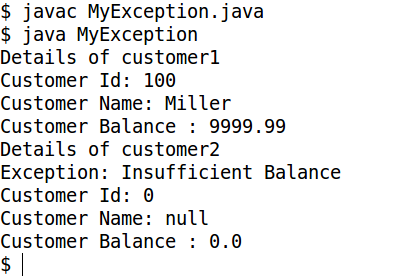
\includegraphics[scale=.5]{throw-example.png}
\end{center}
\end{figure}
\section*{try-with-resources statement}
Java SE 7 provides a new feature \texttt{try-with-resource} statement that will auto close resources.
\begin{lstlisting}[numbers=none]
    System.out.println(``About to open'');
    try(InputStream in = 
     new FileInputStream(``missingfile.txt'')) {
        System.out.println(``File open'');
        int data = in.read();
    } catch(FileNotFoundExceptions e) {
        System.out.println(e.getMessage());
    } catch(IOException e) {
        System.out.println(e.getMessage());
    }
\end{lstlisting}

The \texttt{try-with-resources} statement can eliminate the need for a lengthy finally block. Resources opened using \texttt{try-with-resources} statement are always closed. Any class that implements the \texttt{java.lang.AutoCloseable} can be used as a resource. If a resource should be autocloseable, its reference must be declared within the \texttt{try} statement's parantheses.

Multiple resources can be opened if they are seperated by semocolons. If you open multiple resources, they will be closed in the opposite order in which they are opened.

\section*{Catching Multiple Exceptions}
A single catch block can handle more than one type of exception. This feature can reduce code duplication.

\begin{lstlisting}[numbers=none]
    catch (IOException | SQLException e) {
        System.out.println(e);
    }
\end{lstlisting}
 
\section*{I/O Streams}
\begin{itemize}
\item An I/O Stream represents an input source or an output destination. 
\item A stream can represent many different kinds of sources and destinations like disk files, devices, other programs, a network socket, and memory arrays. 
\item Streams support many different kinds of data like simple bytes, primitive data types, localized characters, and objects. 
\item Some streams simply pass on data, others manipulate and transform the data in useful ways. 
\item No matter how they work internally, all streams present the same simple model to programs that use them. A stream is a sequence of data. 
\end{itemize}

\subsection*{Input Stream}
A program uses an input stream to read data from a source, one item at a time. 

\begin{center}
\begin{figure}[H]
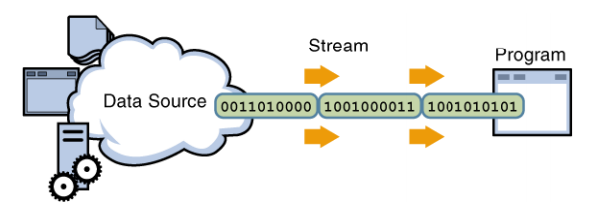
\includegraphics[scale = 0.7]{InputStream.png}
%\caption{Input Stream}
\end{figure}
\end{center}

\subsection*{Output Stream}
A program uses an output stream to write data to a destination, one item at time.

\begin{center}
\begin{figure}[H]
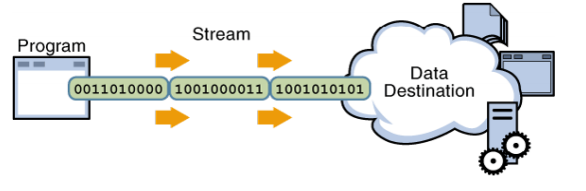
\includegraphics[scale = 0.7]{OutputStream.png}
%%\caption{Output Stream}
\end{figure}
\end{center}
\subsection*{General Stream Types}
The general stream types are: 
\begin{enumerate}
\item \textbf{Character and Byte Streams}
 Character streams are the streams that read and write 16-bit characters whereas Byte streams are the streams that read and write 8-bit bytes.  
\item \textbf{Input and Output Streams}
 Based on source or destination 
\item \textbf{Node and Filter Streams}
 Whether the data on a stream is manipulated or transformed or not. 
\end{enumerate}
\vfill{\ }
\begin{figure}[H]
 \begin{center}
   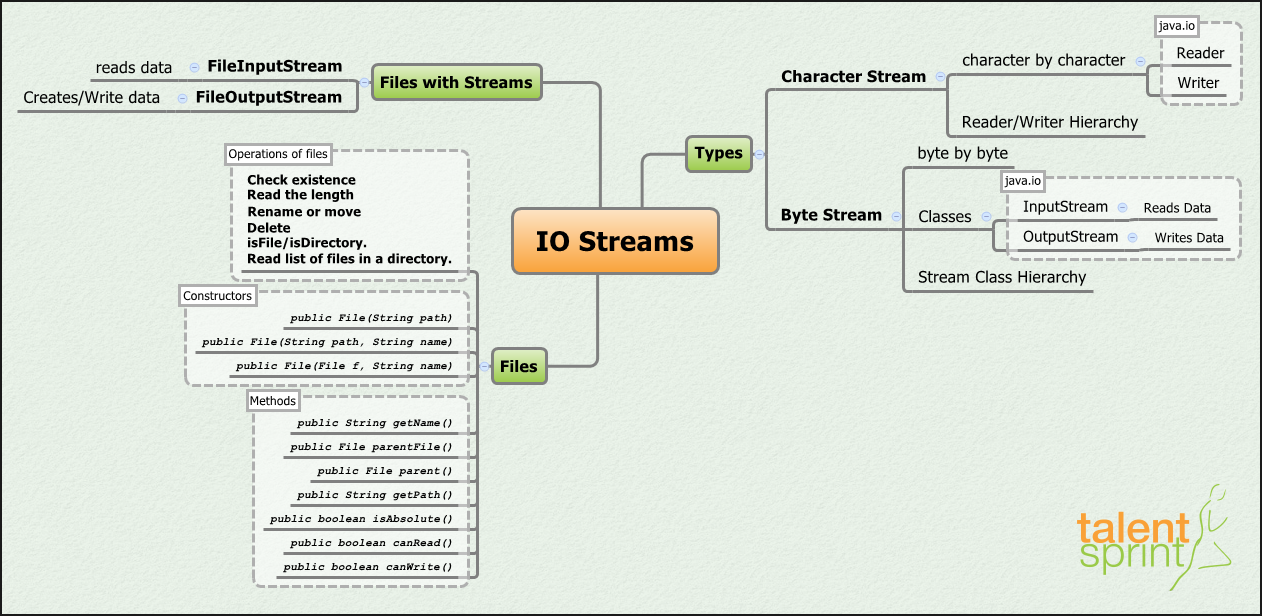
\includegraphics[angle=90,height=20cm, width=13cm]{IOStreams.png}
 \end{center}
 \end{figure}
\subsubsection*{Character and Byte Streams}
\begin{enumerate}
\item \textbf{Byte streams} For binary data, root classes for byte streams are : 
\begin{itemize}
\item The InputStream class 
\item The OutputStream class  
\end{itemize}
\item \textbf{Character streams} For Unicode characters, root classes for character streams are : 
\begin{itemize}
\item The Reader class 
\item The Writer class 
\end{itemize}
\end{enumerate} 
\subsubsection*{Input and Output Streams}
\begin{enumerate}
    \item \textbf{Input or source streams} can read from these streams, root classes of all input streams are : 
        \begin{itemize}
            \item The InputStream class 
            \item The Reader class
                   \end{itemize}
    \item \textbf{Output or sink (destination) streams} Can write to these streams, root classes of all output streams are : 
        \begin{itemize}
            \item The OutputStream class 
            \item The Writer class 
        \end{itemize}
\end{enumerate}

\subsubsection*{Node and Filter Streams}
\begin{enumerate}
\item \textbf{Node streams (Data sink stream)} Contain the basic functionality of reading or writing from a specific location, types of node streams include files, memory, and pipes
\item \textbf{Filter streams (Processing stream)} Layered onto node streams between threads or processes, used for additional functionality like altering or managing data in the stream
\item Adding layers to a node stream is called \texttt{stream chaining}
\end{enumerate}

\subsubsection*{Control Flow of an I/O Operation}
The control flow of an I/O operation is:
\begin{itemize}
    \item Create a stream object and associate it with a data-source (data-destination) 
    \item Give the stream object with the desired functionality through stream chaining 
\end{itemize}
\begin{lstlisting}[numbers=none]
while (there is more information) 
    read(write) next data from(to) the stream 
close the stream
\end{lstlisting}

\subsection*{Byte Stream}
\begin{itemize}
    \item Programs use byte streams to perform input and output of 8-bit bytes. 
    \item All byte stream classes are descended from \texttt{InputStream} and \texttt{OutputStream}. 
    \item There are many byte stream classes like \texttt{FileInputStream} and \texttt{FileOutputStream}. 
    \item They are implemented in the same way, but they differ mainly in the way they are constructed. 
\end{itemize}

\subsection*{When not to use Byte Stream}

Byte Stream represents a kind of low-level I/O that you should avoid: 
\begin{itemize}
    \item If the data contains character data, then the best approach is to use character streams.  
    \item Byte streams should only be used for the most primitive I/O. 
\end{itemize}

\subsection*{Example: FileInputStream and FileOutputStream}
\begin{lstlisting}
public class CopyBytes { 
    public static void main(String[] args) throws IOException { 
        FileInputStream in = null; 
        FileOutputStream out = null; 
        try { 
            in = new FileInputStream(``xanadu.txt''); 
            out = new FileOutputStream(``outagain.txt''); 
            int c; 
            while ((c = in.read()) != -1) { 
                out.write(c); 
            } 
        } 
        finally { 
            if (in != null) { 
                in.close();
            } 
            if (out != null) {
                out.close();
            }
        } 
     }
 } 
 \end{lstlisting}

 \subsection*{Simple Byte Stream Input and Output}
 Simple byte stream input and output is shown in the following diagram: 


 \begin{center}
     \begin{figure}[H]
         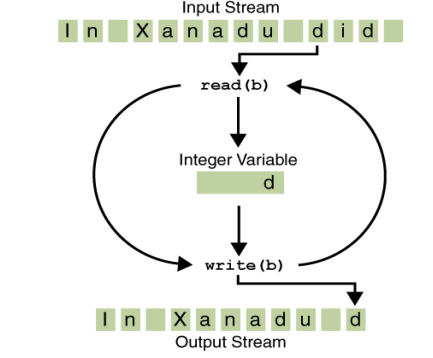
\includegraphics[scale = 0.7]{ByteStream.png}
         %%\caption{Input Stream}
     \end{figure}
 \end{center}

 \subsection*{Character Stream}
 \begin{itemize}
      \item The Java platform stores character values using Unicode conventions. 
      \item Character stream I/O automatically translates the internal format to and from the local character set. In Western locales, the local character set is usually an 8-bit superset of ASCII. 
      \item All character stream classes are descended from \texttt{Reader} and \texttt{Writer}. 
      \item There are character stream classes of \texttt{FileReader} and \texttt{FileWriter} that specialize in file I/O. 
      \item Reader and Writer are the abstract superclasses for character streams in \texttt{java.io} package. 
      \item The \texttt{Reader} and \texttt{Writer} classes were added to JDK 1.1 to support internationalization. 
      \item The Reader and Writer classes make it possible to work with character streams rather than byte streams. 
      \item To a large extent, these character-stream classes mirror the byte stream classes, so if you know how to use one, it isn't too difficult to figure out how to use the other. 
  \end{itemize}

\subsection*{FileReader and FileWriter Example}
\begin{lstlisting}
public class CopyCharacters { 
    public static void main(String[] args) throws IOException { 
        FileReader inputStream = null; 
        FileWriter outputStream = null; 
        try { 
            inputStream = new FileReader(``xanadu.txt''); 
            outputStream = new FileWriter(``characteroutput.txt''); 
            int c; 
            while ((c = inputStream.read()) != -1) { 
                outputStream.write(c); 
            }
        } 
        finally { 
            if (inputStream != null) { 
                inputStream.close(); 
            } 
            if (outputStream != null) { 
                outputStream.close(); 
            } 
        } 
    } 
}
\end{lstlisting}
\subsection*{Character Stream and Byte Stream}
\begin{itemize}
    \item Character streams are often ``wrappers'' for byte streams. 
    \item The character stream uses the byte stream to perform the physical I/O, while the character stream handles translation between characters and bytes. \texttt{FileReader}, for example, uses \texttt{FileInputStream}, while \texttt{FileWriter} uses \texttt{FileOutputStream}.
\end{itemize}
\subsection*{Line-Oriented I/O}
\begin{itemize}
    \item Character I/O usually occurs in bigger units than single characters: 
    \item For the line-oriented I/O, one common single unit is the line that contains a string of characters with a line terminator at the end. 
    \item A line terminator can be a carriage-return or linefeed sequence (``\textbackslash r\textbackslash n''), a single carriage-return (``\textbackslash r''), or a single line-feed (``\textbackslash n''). 
\end{itemize}

\subsection*{Line-oriented I/O Example}
\begin{lstlisting}[numbers=none]
File inputFile = new File(``farrago.txt''); 
File outputFile = new File(``outagain.txt''); 
FileReader in = new FileReader(inputFile); 
FileWriter out = new FileWriter(outputFile); 
BufferedReader inputStream = new BufferedReader(in); 
PrintWriter outputStream = new PrintWriter(out); 
String l; 
while ((l = inputStream.readLine()) != null) { 
     System.out.println(l); 
      outputStream.println(l); 
} 
in.close(); 
out.close(); 
\end{lstlisting}

\subsection*{Buffered Streams}
\begin{itemize}
    \item An unbuffered I/O means each read or write request is handled directly by the underlying OS. This can make a program much less efficient, because each such request often triggers disk access, network activity, or some other operation that is relatively expensive.
\item To reduce this kind of overhead, the Java platform implements buffered I/O streams:
\item Buffered input streams read data from a memory area known as a buffer. The native input API is called only when the buffer is empty
\item Similarly, buffered output streams write data to a buffer, and the native output API is called only when the buffer is full. 
\end{itemize}


\subsubsection*{How to Create Buffered Streams?}
\begin{itemize}
    \item A program can convert an unbuffered stream into a buffered stream using the wrapping idiom. An unbuffered stream object is passed to the constructor for a buffered stream class.
    \end{itemize} 
\textbf{Example:} 
\begin{lstlisting}[numbers=none]
inputStream = new BufferedReader(new FileReader(``xanadu.txt'')); 
outputStream = new BufferedWriter(new 
FileWriter(``characteroutput.txt'')); 
\end{lstlisting}


\subsubsection*{Buffered Stream Classes}
\begin{itemize}
    \item \texttt{BufferedInputStream} and \texttt{BufferedOutputStream} create buffered byte streams. 
    \item \texttt{BufferedReader} and \texttt{BufferedWriter} create buffered character streams. 
\end{itemize}

\subsubsection*{Flushing Buffered Streams}
\begin{itemize}
    \item It often makes sense to write out a buffer at critical points, without waiting for it to fill. This is known as flushing the buffer
    \item Some buffered output classes support autoflush, specified by an optional constructor argument: 
    \item When autoflush is enabled, certain key events cause the buffer to be flushed.
    \item For example, an autoflush \texttt{PrintWriter} object flushes the buffer on every invocation of println or format. 
    \item To flush a stream manually, invoke its flush method. The flush method is valid on any output stream, but has no effect unless the stream is buffered. 
\end{itemize}

\subsection*{Standard Streams on Java Platform}
\begin{itemize}
    \item Three standard streams on Java platform are: 
        \begin{itemize}
            \item Standard Input, accessed through System.in 
            \item Standard Output, accessed through System.out 
            \item Standard Error, accessed through System.err 
        \end{itemize}
    \item These objects are defined automatically and do not need to be opened. 
    \item \texttt{System.out} and \texttt{System.err} are defined as \texttt{PrintStream} objects
\end{itemize}
\subsection*{Data Streams}
\begin{itemize}
    \item Data streams support binary I/O of primitive data type values (boolean, char, byte, short, int, long, float, and double) as well as String values. 
    \item All data streams implement either the \texttt{DataInput} interface or the \texttt{DataOutput} interface. 
    \item \texttt{DataInputStream} and \texttt{DataOutputStream} are the implementations that are applied most widely of these interfaces. 
\end{itemize}

\subsubsection*{DataOutputStream}
\texttt{DataOutputStream} can only be created as a wrapper for an existing byte stream object. 
\begin{lstlisting}[numbers=none, xleftmargin=.25in]
out = new DataOutputStream(new BufferedOutputStream( 
      new FileOutputStream(dataFile))); 
for (int i = 0; i < prices.length; i ++) { 
    out.writeDouble(prices[i]); 
    out.writeInt(units[i]);
    out.writeUTF(descs[i]); 
} 
\end{lstlisting}


\subsubsection*{DataInputStream}
\begin{itemize}
    \item Like DataOutputStream, DataInputStream must be constructed as a wrapper for a byte stream
    \item End-of-file condition is detected by catching EOFException, instead of testing for an invalid return value.
\end{itemize}
\begin{lstlisting}[numbers=none, xleftmargin=.25in]
in = new DataInputStream(new BufferedInputStream( 
     new FileInputStream(dataFile))); 
try { 
    double price = in.readDouble(); 
    int unit = in.readInt(); 
    String desc = in.readUTF(); 
} catch (EOFException e) { 

} 
\end{lstlisting}

\subsection*{The File Class}
\begin{itemize}
    \item The \texttt{File} class is not a stream class. 
    \item The \texttt{File} class is important because stream classes manipulate File objects. 
    \item The \texttt{File} class is an abstract representation of actual files and directory pathname. 
\end{itemize}

\subsection*{The File Class Example}
\begin{lstlisting}
import java.io.*; 
public class FileInfoClass { 
    public static void main(String args[]) { 
        String fileName = args[0]; 
        File fn = new File(fileName); 
        System.out.println(``Name: '' + fn.getName()); 
        if (!fn.exists()) { 
            System.out.println(fileName + 
                      `` does not exists.''); 
            
            /* Create a temporary directory instead. */ 
            
            System.out.println("Creating temp directory"); 
            fileName = ``temp'';
            fn = new File(fileName); 
            fn.mkdir(); 
            System.out.println(fileName + (fn.exists() ``exists'': ``does not exist'')); 
            System.out.println(``Deleting temp directory''); 
            fn.delete(); 
            System.out.println(fileName + `` is a '' + fn.isFile() ``file.'' :``directory.'')); 
            if (fn.isDirectory()) { 
                String content[] = fn.list(); 
                System.out.println(``The content of 
                       this directory:'');
                for (int i = 0; i < content.length; i++) {
                    System.out.println(content[i]); 
                } 
            } 
            if (!fn.canRead()) { 
                System.out.println(fileName + `` is not readable.''); 
                return;
            } 
            System.out.println(fileName + `` is '' +fn.length() + `` bytes long.''); 
            System.out.println(fileName + `` is '' +fn.lastModified() + `` bytes long.''); 
            if (!fn.canWrite()) { 
                System.out.println(fileName + `` is not writable.''); 
            } 
        } 
    }
}
\end{lstlisting}

\subsection*{Example}
Write a program that illustrates the usage of \texttt{InputStreamReader} and \texttt{BufferedReader} classes that are used to convert the standard input stream (System.in) from a byte stream to a character stream

\begin{lstlisting}
import java.io.*; 
public class InputConversionApp { 
    public static void main(String args[]) throws IOException { 
        InputStreamReader in = new InputStreamReader(System.in); 
        BufferedReader inStream = new BufferedReader(in); 
        System.out.println(``Encoding: '' + in.getEncoding()); 
        String inputLine; 
        do { 
            System.out.print(``>''); 
            System.out.flush(); 
            inputLine = inStream.readLine(); 
            System.out.println(inputLine); 
        } while (inputLine.length() != 0); 
    } 
}
\end{lstlisting} 
\subsection*{How It Works:}
\begin{itemize}
    \item The InputConversionApp program converts the standard input stream (System.in) from a byte stream to a character stream.    \item The input characters are echoed to standard output.
    \item The program also prints out the encoding that is in effect on your system.
\end{itemize}

\subsection*{Serialization}
\begin{itemize}
    \item Serialization is an ability to read or write an object to a stream. It is the process of ``flattening'' an object. 
    \item Serialization is used to save object to some permanent storage. Its state should be written in a serialized form to a file such that the object can be reconstructed at a later time from that file. 
    \item Serialization is used to pass on to another object by the OutputStream class and can be sent over the network. 
\end{itemize}

\subsubsection*{Streams Used for Serialization}
The streams used for serialization are: 
\begin{description}
    \item [ObjectOutputStream]  For serializing (flattening an object) 
    \item [ObjectInputStream]  For deserializing (reconstructing an object) 
\end{description}
\begin{figure}[H]
 \begin{center}
   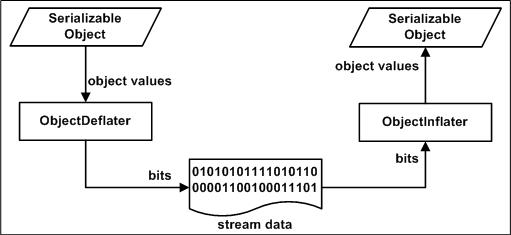
\includegraphics[scale=0.8]{serialization.jpg}
   \caption{Serialization and Deserialization}
 \end{center}
 \end{figure}
\subsubsection*{Requirement for Serialization}
\begin{itemize}
    \item Serialization is required to allow an object to be serializable 
    \item Its class should implement the \texttt{Serializable} interface
        \begin{itemize}
            \item \texttt{Serializable} interface is marker interface
            \item Its class should also provide a default constructor (a constructor with no arguments) 
        \end{itemize}
    \item Serializability is inherited 
        \begin{itemize}
            \item Do not have to implement Serializable on every class 
            \item Can just implement Serializable once along the class hierarchy 
        \end{itemize}
\end{itemize}

\subsubsection*{Non-Serializable Objects}
\begin{itemize}
    \item Most Java classes are serializable. 
    \item Objects of some system-level classes are not serializable: 
    \item Because the data that they represent, changes constantly: 
    \item Reconstructed object will contain different value anyway 
    \item For example, thread running in your JVM would be applying the memory of your system. Persisting it and trying to run it in your JVM would make no sense at all
    \item A \texttt{NotSerializableException} is thrown if you try to serialize non-serializable objects
\end{itemize}

\subsection*{What is Preserved when an Object is Serialized?}
When an object is serialized enough information is preserved that is needed to reconstruct the object instance at a later time:
\begin{itemize}
    \item Only the data of the object is preserved 
    \item Methods and constructors are not part of the serialized stream 
    \item Class information is included 
\end{itemize}

\subsubsection*{The transient Keyword}
\begin{itemize}
    \item The \texttt{transient} modifier applies only to instance variables. 
    \item If you mark an instance variable as \texttt{transient}, you are telling the JVM to skip (ignore) this variable when you attempt to serialize the object containing it. 
    \item In other words, the \texttt{transient} keyword prevents the data from being serialized. 
    \item All fields that are not \texttt{transient} are considered part of the persistent state of an object and are eligible for persistence.
\end{itemize}

\subsection*{Serialization: Writing an Object Stream}
To write an object stream use its writeObject method of the ObjectOutputStream class. 
\begin{lstlisting}[numbers=none]
public final void writeObject(Object obj) throws IOException
\end{lstlisting}

where obj is the object to be written to the stream
\lstinputlisting{../Code/Employee.java}
\lstinputlisting{../Code/SerializeDemo.java}

\subsection*{Deserialization: Reading an Object Stream}
To read an object stream use its \texttt{readObject} method of the \texttt{ObjectInputStream} class. 
\begin{lstlisting}[numbers=none]
public final Object readObject() throws IOException, 
                      ClassNotFoundException
\end{lstlisting}

where \texttt{`obj'} is the object to be read from the stream 

The Object type returned should be typecasted to the appropriate class name before methods on that class can be executed. 
\lstinputlisting{../Code/DeserializeDemo.java}

\end{document}


